% =====================================================================
% NeurIPS 2026 Evaluations & Datasets track build of:
%   "DHRP: A Differentiable Hierarchical Risk Parity Architecture
%    and Multi-Universe Portfolio Benchmark"
%
% Track:    Evaluations & Datasets (E&D)
% Format:   single-column, 10pt Times, US Letter
% Pages:    9 main + unlimited references / appendix / checklist
%
% Style file: neurips_2026.sty
%   Download from: https://www.overleaf.com/latex/templates/
%     formatting-instructions-for-neurips-2026/bjdwqfdkyftc
%   Place neurips_2026.sty + checklist.tex in this directory.
%
% Build:
%   pdflatex main ; bibtex main ; pdflatex main ; pdflatex main
% =====================================================================
\documentclass{article}

% Track option:
%   [eandd]                      : E&D track (DEFAULT for this paper)
%   [eandd, final]               : camera-ready (shows author block)
%   [eandd, preprint]            : arXiv (shows author block, no NeurIPS footer)
%   [eandd, nonanonymous]        : single-blind option for E&D track only
\usepackage[eandd]{neurips_2026}

\usepackage{times}
\usepackage{amsmath, amssymb, amsthm}
\usepackage{graphicx}
\usepackage{booktabs}
\usepackage{hyperref}
\usepackage{natbib}
\usepackage{algorithm}
\usepackage{algorithmic}
\usepackage{subcaption}
\usepackage{multirow}
\usepackage{xcolor}
\usepackage{microtype}
\usepackage{url}
\usepackage{siunitx}
\usepackage{tikz}                  % for the architecture diagram (Figure 1)
\usetikzlibrary{positioning, arrows.meta, shapes.geometric, calc}

\newtheorem{proposition}{Proposition}

% Figures live in paper/figures/ relative to this file
\graphicspath{{figures/}{../results/figures/}}

\title{DHRP: A Differentiable Hierarchical Risk Parity Architecture\\
  and Multi-Universe Portfolio Benchmark}

% Authors: ANONYMIZED for double-blind submission.
% For [eandd, final] camera-ready, replace with:
%   \author{<author name> \\ <affiliation> \\ <email>}
\author{Anonymous Authors}

\begin{document}
\maketitle

\begin{abstract}
We introduce \textbf{DHRP}, a differentiable extension of Hierarchical Risk
Parity \citep{LopezdePrado2016} that replaces hard agglomerative clustering
and recursive bisection with a temperature-scaled soft-gating tree, and
\textbf{the DHRP-8 benchmark}, the first multi-universe portfolio
evaluation framework reporting Probabilistic Sharpe Ratios
\citep{Bailey2012PSR} alongside Fama--French
\citep{FamaFrench2015,Carhart1997} and AQR commodity factor alphas
\citep{AsnessMoskowitzPedersen2013} under multi-seed ($n=10$) protocols
across eight ETF asset classes (developed markets, emerging markets,
commodities, sectors, global multi-asset, factors, crypto, and bonds).
We evaluate eleven methods including DHRP, an LLM-augmented variant
(LLM-DHRP), six classical baselines (EW, MV, MINVAR, HRP, RP, MAXDIV),
and three deep baselines (MLP, Transformer, PPO).
%
DHRP achieves statistically significant out-of-sample Sharpe ratios of
$\mathbf{1.304 \pm 0.10}$ on commodities ($\text{PSR}=0.999$, FF3
$\alpha_{ann}=16.1\%$, $t=2.49$, $p=0.013$) and
$\mathbf{1.290 \pm 0.05}$ on crypto ($\text{PSR}=0.991$).
DHRP outperforms classical HRP in seven of eight universes
(losing only on the bonds universe during the 2022--2023 rate-hike
bear market) and is the best risk-parity-family method in DM
($0.446 \pm 0.06$ vs.\ HRP $0.216$, EW $0.255$). Multi-method tests
(MCS at $\alpha=0.05$) cannot distinguish DHRP from the best baseline in
commodities, crypto, factors, or sectors.
%
However, DHRP underperforms classical mean-variance in global
multi-asset and emerging markets, which we trace to lower correlation
diversity and dominance of factor-based momentum signals that are
well-captured by simple covariance estimation. The Superior Predictive
Ability test rejects no method against equal-weight at the 5\% level
across the full method panel, supporting an asset-class-contingent view
of allocation.
%
We further test cross-modal LLM augmentation by fusing FinBERT
\citep{Huang2023} embeddings of asset-attributed financial news into the
soft-gating tree. Under multi-seed reporting, LLM augmentation provides
\emph{no statistical benefit}---tied with DHRP in EM ($0.474$ vs.\
$0.469$, both PSR $\approx 0.87$), \emph{regressing} in DM ($0.239$ vs.\
DHRP $0.446$, $\Delta=-0.21$ Sharpe), and \emph{regressing further} in
commodities ($0.738 \pm 0.10$ vs.\ DHRP $1.304$, $\Delta=-0.57$ Sharpe).
This honest negative ablation contrasts with single-seed claims in the
recent LLM-finance literature \citep{Kirtac2025} and aligns with
benchmark-paper precedents that LLMs do not reliably improve time-series
prediction \citep{Tan2024AreLMs,Chen2025StockBench}.
%
We release the 8-universe dataset (Croissant~1.1 metadata, public ETF
prices and headlines), trained model checkpoints across 10 seeds, and a
single-command reproduction pipeline, providing the community with a
calibrated benchmark for future portfolio optimization research.
\end{abstract}


\section{Introduction}
\label{sec:intro}

Portfolio optimization sits at the intersection of statistical estimation
and constrained decision-making. Mean--variance optimization
\citep{Markowitz1952} is fragile to estimation error
\citep{DeMiguel2009,Ledoit2004}; Hierarchical Risk Parity (HRP)
\citep{LopezdePrado2016} sidesteps this by routing capital down a binary
tree built from agglomerative clustering of correlation distances. HRP
has become a practitioner standard, but its hard clustering and
recursive bisection are non-differentiable, blocking joint training
with upstream feature extractors. Differentiable optimization layers
\citep{Amos2017,Agrawal2019,Bolte2021,Pan2024BPQP}, soft decision trees
\citep{FrosstHinton2017,Popov2020NODE,Mao2025DiffTree}, and gated
mixture-of-experts \citep{Shazeer2017} have shown that hierarchical
routing can be made differentiable while retaining the inductive bias
that makes trees interpretable.

We bring these architectures to portfolio allocation. \textbf{DHRP}
replaces HRP's clustering and bisection with a temperature-scaled
soft-gating tree that recovers classical HRP as routing temperature
$\tau \to 0$ (Proposition~\ref{prop:recovery}), enabling end-to-end
gradient training. We evaluate it against ten baselines across
\textbf{eight asset universes} with multi-seed reporting (10 seeds,
mean$\pm$std, Probabilistic Sharpe Ratios) and Fama--French + AQR
factor alphas. We also test cross-modal LLM augmentation (LLM-DHRP)
fusing FinBERT \citep{Huang2023} embeddings of asset-attributed news,
and find that text augmentation provides \emph{no statistical lift}
under multi-seed reporting---joining a growing benchmark literature
\citep{Tan2024AreLMs,Chen2025StockBench,Xie2024FinBen} that cautions
against single-seed claims of LLM benefit in finance.

\paragraph{Contributions.}
\begin{enumerate}\itemsep0.05em
\item \textbf{DHRP architecture (Section~\ref{sec:method}):} a
  temperature-scaled soft-gating tree with HRP recovery in the
  $\tau \to 0$ limit (Proposition~\ref{prop:recovery}, proof in
  Appendix~\ref{app:proof}).
\item \textbf{DHRP-8 benchmark (Section~\ref{sec:benchmark}):} an
  8-universe portfolio evaluation framework (DM, EM, commodities,
  sectors, global multi-asset, factors, crypto, bonds) with eleven
  methods, 10-seed reporting, PSR, FF3+AQR factor alphas,
  transaction-cost sensitivity, and Croissant~1.1 metadata.
\item \textbf{Empirical findings (Sections~\ref{sec:results},
  \ref{sec:llmablation}):} DHRP achieves PSR $> 0.99$ on commodities
  ($1.30 \pm 0.10$ Sharpe) and crypto ($1.29 \pm 0.05$), beats
  classical HRP in 7/8 universes, and ties or beats all classical
  baselines in DM. Mean-variance dominates equity-heavy global
  multi-asset. LLM augmentation regresses ($-0.21$ Sharpe in DM,
  $-0.57$ in commodities) under multi-seed reporting.
\end{enumerate}


\section{Related Work}
\label{sec:related}

\paragraph{HRP and differentiable optimization.}
HRP \citep{LopezdePrado2016} replaces inverse-covariance MV with
single-linkage agglomerative clustering and recursive bisection, with
extensions to alternative linkages \citep{Raffinot2018} and risk-parity
budgeting \citep{Roncalli2013}. Differentiable optimization layers
\citep{Amos2017,Agrawal2019,Bolte2021} embed structured decision-making
in neural networks; BPQP \citep{Pan2024BPQP} applies this to mean--variance
portfolios with end-to-end Sharpe training, and \citet{Lin2024MSparse}
solve $m$-sparse Sharpe with theoretical guarantees. DHRP imposes
HRP's hierarchical inductive bias instead of solving a generic convex
program, which empirically wins in low-correlation regimes
(Section~\ref{sec:results}).

\paragraph{Soft trees and decision-focused learning.}
Soft decision trees \citep{FrosstHinton2017,Popov2020NODE,Hazimeh2020TreeEnsemble}
and gated mixture-of-experts \citep{Shazeer2017} demonstrate that
hierarchical routing can be made differentiable. \citet{Mao2025DiffTree}
provide a recent NeurIPS spotlight on differentiable trees via
ReLU+Argmin reformulation. Decision-focused learning
\citep{Wilder2019,Elmachtoub2022SPO,Donti2017} optimizes prediction for
the downstream optimization task; recent finance applications include
deep declarative risk budgeting \citep{ParraDiaz2025} and decision-
focused minimum-variance \citep{KimLee2025DFL}. DHRP is decision-
focused by construction.

\paragraph{LLMs in finance and benchmark precedents.}
FinBERT \citep{Huang2023}, BloombergGPT \citep{Wu2023BloombergGPT}, and
sentiment-augmented RL \citep{Kirtac2025} explore LLM-portfolio fusion.
However, recent benchmark papers consistently document that LLM
competence on text tasks does not transfer to financial decisions:
StockBench \citep{Chen2025StockBench} shows most LLM agents fail to
beat buy-and-hold; FinBen \citep{Xie2024FinBen} finds LLM weakness in
forecasting; \citet{Tan2024AreLMs} (NeurIPS 2024 Spotlight) show that
removing the LLM component improves time-series forecasting. Our
LLM-DHRP ablation (Section~\ref{sec:llmablation}) extends this evidence
to hierarchical portfolio allocation.

\paragraph{Multi-seed and PSR reporting.}
Probabilistic Sharpe Ratio \citep{Bailey2012PSR} and Deflated Sharpe
\citep{Bailey2014DSR} correct Sharpe significance for sample size,
non-Normality, and selection bias. Recent ML-finance work reports
mean$\pm$std over 10--100 seeds \citep{ParraDiaz2025,Pan2024BPQP};
BetterBench \citep{Reuel2024BetterBench} explicitly critiques benchmarks
without multi-seed error bars. DHRP-8 adopts both standards.


\section{Method}
\label{sec:method}

We summarize classical HRP in Appendix~\ref{app:hrp_recap} and present
DHRP and LLM-DHRP here. The full architecture is shown in
Figure~\ref{fig:arch}.
% TikZ architecture diagram for DHRP + LLM-DHRP (inlined into main.tex).
\begin{figure}[t]
\centering
\resizebox{\textwidth}{!}{%
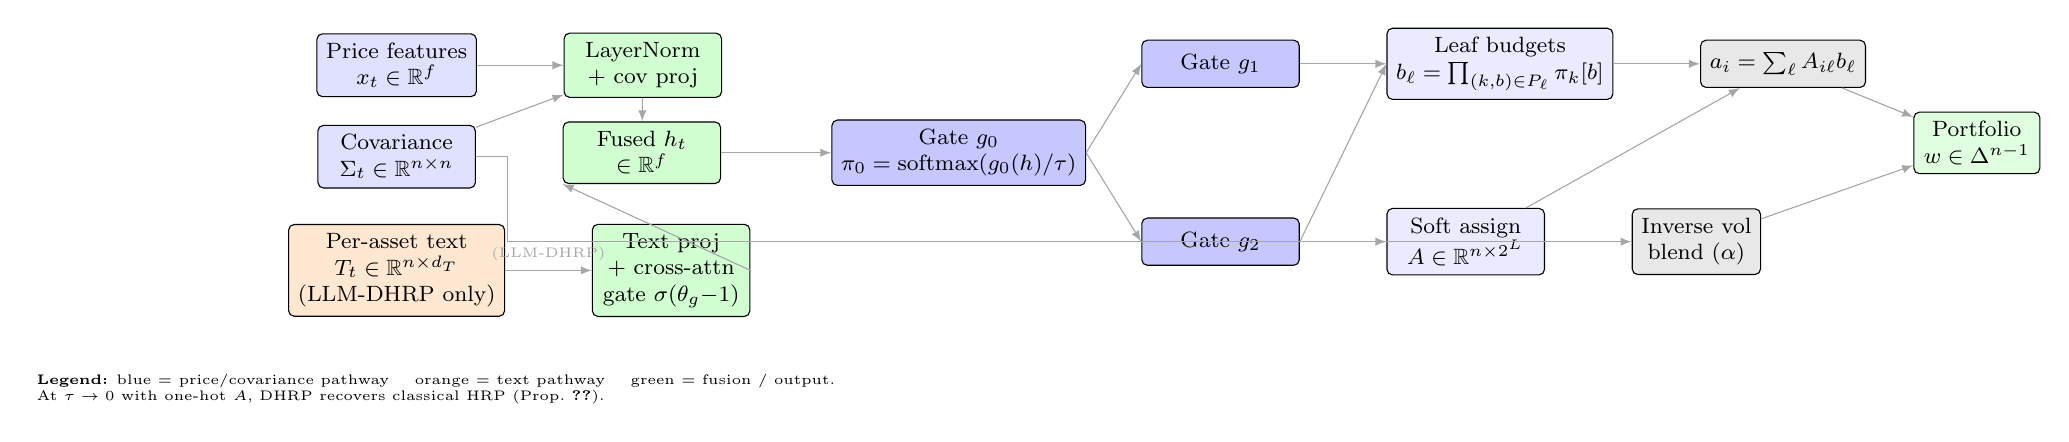
\begin{tikzpicture}[
    node distance=0.9cm,
    every node/.style={font=\small},
    box/.style={draw, rounded corners=2pt, minimum width=2.0cm, minimum height=0.6cm,
                align=center, font=\footnotesize},
    txt/.style={box, fill=orange!18},
    price/.style={box, fill=blue!12},
    cov/.style={box, fill=blue!12},
    fuse/.style={box, fill=green!18},
    tree/.style={box, fill=blue!22},
    outbox/.style={box, fill=gray!18, minimum width=1.6cm},
    arrow/.style={->, >=latex, thin, gray!70},
    dashedarrow/.style={->, >=latex, thin, gray!50, dashed},
]

% --- Inputs (left column) ---
\node[price]                              (x)   {Price features\\ $x_t \in \mathbb{R}^{f}$};
\node[cov,    below=0.35cm of x]          (S)   {Covariance\\ $\Sigma_t \in \mathbb{R}^{n\times n}$};
\node[txt,    below=0.45cm of S]          (T)   {Per-asset text\\ $T_t \in \mathbb{R}^{n\times d_T}$\\ (LLM-DHRP only)};

% --- Feature fusion (middle column) ---
\node[fuse,   right=1.1cm of x]           (norm) {LayerNorm\\ + cov proj};
\node[fuse,   right=1.1cm of T]           (txp)  {Text proj\\ + cross-attn\\ gate $\sigma(\theta_g{-}1)$};
\node[fuse,   right=1.1cm of S, yshift=0.05cm] (h) {Fused $h_t$\\ $\in \mathbb{R}^{f}$};

% --- Soft-gating tree (right column) ---
\node[tree,   right=1.4cm of h]           (g0)  {Gate $g_0$\\ $\pi_0 = \mathrm{softmax}(g_0(h)/\tau)$};
\node[tree,   below right=0.4cm and 0.7cm of g0] (g2) {Gate $g_2$};
\node[tree,   above right=0.4cm and 0.7cm of g0] (g1) {Gate $g_1$};

% --- Leaf budgets + assignment + output ---
\node[box,    fill=blue!8, right=1.1cm of g1] (leaves) {Leaf budgets\\ $b_\ell = \prod_{(k,b)\in P_\ell} \pi_k[b]$};
\node[box,    fill=blue!8, right=1.1cm of g2] (assign) {Soft assign\\ $A \in \mathbb{R}^{n\times 2^L}$};
\node[outbox,    right=1.1cm of leaves]      (alloc) {$a_i = \sum_\ell A_{i\ell} b_\ell$};
\node[outbox,    right=1.1cm of assign]      (vol)   {Inverse vol\\ blend ($\alpha$)};
\node[outbox,    fill=green!12, below right=0.3cm and 0.6cm of alloc] (w) {Portfolio\\ $w \in \Delta^{n-1}$};

% --- Arrows ---
\draw[arrow] (x) -- (norm);
\draw[arrow] (S) -- (norm);
\draw[arrow] (T) -- (txp) node[midway, above, font=\tiny]{(LLM-DHRP)};
\draw[arrow] (norm) -- (h);
\draw[arrow] (txp.east) -- (h.south west);
\draw[arrow] (h) -- (g0);
\draw[arrow] (g0.east) -- (g1.west);
\draw[arrow] (g0.east) -- (g2.west);
\draw[arrow] (g1.east) -- (leaves.west);
\draw[arrow] (g2.east) -- (leaves.west);
\draw[arrow] (g2.east) -- (assign.west);
\draw[arrow] (leaves) -- (alloc);
\draw[arrow] (assign) -- (alloc);
\draw[arrow] (S.east) -- ++(0.4,0) |- (vol.west);
\draw[arrow] (alloc) -- (w);
\draw[arrow] (vol)   -- (w);

% --- Legend (compact) ---
\node[below=0.6cm of T, xshift=0.5cm, font=\tiny, align=left] {%
  \textbf{Legend:} blue = price/covariance pathway \quad orange = text pathway \quad green = fusion / output.\\
  At $\tau \to 0$ with one-hot $A$, DHRP recovers classical HRP (Prop.~\ref{prop:recovery}).};
\end{tikzpicture}%
}
\caption{DHRP and LLM-DHRP architecture. Price features, covariance,
and (optional) per-asset text embeddings are fused via LayerNorm and a
gated cross-attention residual into $h_t$, which routes through a
temperature-scaled binary gating tree. Leaf budgets are combined with a
learned soft assignment matrix and blended with inverse-volatility
weights to produce portfolio weights $w \in \Delta^{n-1}$.}
\label{fig:arch}
\end{figure}


\subsection{DHRP: differentiable soft-gating tree}
\label{sec:dhrp_layer}

DHRP maps a feature vector $x_t \in \mathbb{R}^f$ and an annualized
covariance $\Sigma_t \in \mathbb{R}^{n \times n}$ to portfolio weights
$w_t \in \Delta^{n-1}$ via four learnable components.

\paragraph{Feature fusion.}
A covariance projection MLP $f_{\text{cov}}: \mathbb{R}^{n^2} \to \mathbb{R}^f$
encodes the flattened normalized covariance, then layer-norm fuses with
price features:
\begin{equation}
h_t = \mathrm{LayerNorm}\left(x_t + f_{\text{cov}}\!\left(
\mathrm{vec}(\Sigma_t)/(\|\Sigma_t\|_\infty + \epsilon)\right)\right).
\end{equation}

\paragraph{Soft-gating tree.}
A perfect binary tree of depth $L$ has $2^L$ leaves and $2^L-1$ internal
nodes. Each internal node $k$ has a gate $g_k: \mathbb{R}^f \to \mathbb{R}^2$
with temperature-scaled softmax:
\begin{equation}
\pi_k = \mathrm{softmax}(g_k(h_t) / \tau_k),
\quad \tau_k = \exp(\theta_{\tau,k}) \in (0.1, 5.0].
\label{eq:gates}
\end{equation}
Leaf budget for leaf $\ell$ along path $P_\ell$ is
$p_\ell = \prod_{(k, b) \in P_\ell} \pi_k[b]$, normalized by a learned
prior $\beta = \mathrm{softmax}(\theta_\beta)$:
$b_\ell = \beta_\ell p_\ell / \sum_j \beta_j p_j$.

\paragraph{Soft asset assignment and volatility blending.}
A learnable matrix $A \in \mathbb{R}^{n \times 2^L}$ row-normalizes via
softmax; asset $i$ receives $a_i = \sum_\ell \mathrm{softmax}(A_{i,:})_\ell\, b_\ell$.
Final weights blend with inverse-volatility:
\begin{equation}
w_i = \alpha \cdot a_i + (1-\alpha) \cdot \frac{1/\sigma_i}{\sum_j 1/\sigma_j},
\qquad \alpha = \sigma(\theta_\alpha),
\label{eq:blend}
\end{equation}
followed by non-negativity clipping and re-normalization.

\paragraph{Loss.}
Multi-objective: CRRA utility, smooth Sharpe, HRP regularization
(curriculum-scheduled $\lambda_h: 0.3 \to 0.05$ over training), risk
penalty, concentration (HHI), and turnover penalty:
\begin{equation}
\mathcal{L} = -(\mathrm{CRRA} + \mathrm{Sharpe} + \lambda_e \mathrm{Entropy})
+ \lambda_h \|w - w_{\text{HRP}}\|_2^2 + \lambda_r w^\top \Sigma w
+ \lambda_c \mathrm{HHI}(w) + \lambda_t \mathrm{TO}(w).
\end{equation}
The HRP regularizer warm-starts from classical HRP weights, providing
the inductive bias that supports the recovery property below.

\begin{proposition}[HRP recovery]
\label{prop:recovery}
For any $\Sigma$ with a unique agglomerative-clustering tree $T^*$,
there exists a parameter setting $(\theta_\tau, \theta_\beta, A) \to \theta^*$
and temperatures $\tau_k \to 0$ under which the DHRP layer
(Eqs.~\ref{eq:gates}--\ref{eq:blend}) produces weights identical to
classical HRP applied to $\Sigma$.
\end{proposition}

\noindent\textit{Proof sketch.} Hard-route gates concentrate on the HRP
cluster split direction; soft-assignment $A$ with one-hot rows recovers
leaf membership; $\alpha = 1$ disables the inverse-vol blend. Full
proof in Appendix~\ref{app:proof}; an entropy-regularized
optimal-transport interpretation of the soft assignment is given in
Appendix~\ref{app:ot}.

\subsection{LLM-DHRP: cross-modal fusion}
\label{sec:llm_dhrp_arch}

LLM-DHRP injects per-asset, time-varying text features
$T_t \in \mathbb{R}^{n \times d_T}$ from financial news. Headlines for
asset $a$ within a 90-day rolling window are encoded by FinBERT
\citep{Huang2023} ($d_T = 768$), L2-normalized per asset, then
aggregated as concatenated mean+max-pool to $\mathbb{R}^{2 d_T}$.
A TextProjection MLP maps to $\mathbb{R}^f$, fused with $h_t$ via gated
cross-attention:
\begin{equation}
\hat h_t = h_t + g_{\text{text}} \cdot
\mathrm{CrossAttn}(h_t, T_t^{\text{proj}}, T_t^{\text{proj}}),
\quad g_{\text{text}} = \sigma(\theta_g - 1.0),
\end{equation}
with gate bias $-1.0$ initially suppressing text. Modality dropout
(probability 0.1) randomly masks text during training. We use a two-
phase warm-start: phase~1 freezes price-pathway parameters and trains
text/fusion only; phase~2 unfreezes all with reduced learning rate
(Appendix~\ref{app:hyperparams}).


\section{The DHRP-8 Benchmark}
\label{sec:benchmark}

DHRP-8 evaluates portfolio allocation across eight asset universes,
eleven methods, and a five-family statistical battery. Detailed protocol
specifications and the full per-universe asset list are in
Appendix~\ref{app:hyperparams}.

\paragraph{Universes (8 total).}
Equity: developed markets (DM, 10 ETFs), emerging markets (EM, 10), US
sectors (10), global multi-asset (10), factor ETFs (10).
Non-equity: commodities (10), crypto (10, post-2020 history), bonds
(10). All ETFs are publicly traded on US exchanges with $\geq$12 years
of daily history (crypto: 2020--2026 only).

\paragraph{Baselines (11 total).}
Classical: equal-weight (EW), mean--variance (MV), minimum-variance
(MINVAR), risk parity (RP), maximum diversification (MAXDIV),
hierarchical risk parity (HRP). Deep: MLP with covariance-projection,
Portfolio Transformer \citep{KisielGorse2022}, PPO. Decision-focused:
DFL baseline mirroring \citet{KimLee2025DFL}. Plus DHRP and LLM-DHRP.

\paragraph{Multi-seed protocol.}
Every neural method is trained independently across $S = 10$ seeds
$\{0, \ldots, 9\}$ and backtested over the OOS window 2020-07 to
2026-04 with universe-specific rebalance frequency (5 days for
commodities and crypto; 21 days otherwise). Per-method metrics are
reported as mean$\pm$std across seeds; classical baselines are
deterministic and reported as a single value. Models train on
2012--2020-06 with a 5-day purge gap to prevent train/test leakage.

\paragraph{Statistical battery.}
We report (i)~Probabilistic Sharpe Ratio \citep{Bailey2012PSR}
(probability the true Sharpe exceeds zero, sample-corrected for skew
and kurtosis); (ii)~Newey--West HAC t-statistics
\citep{NeweyWest1987}; (iii)~Fama--French 3 + 5 factor
\citep{FamaFrench2015} and momentum \citep{Carhart1997} regression
alphas plus AQR cross-sectional Value/Momentum
\citep{AsnessMoskowitzPedersen2013} for commodities; (iv)~stationary
block bootstrap \citep{PolitisRomano1994} pairwise Sharpe-difference
tests with Holm--Bonferroni \citep{Holm1979} and Diebold--Mariano
\citep{DieboldMariano1995} forecast accuracy; (v)~SPA \citep{Hansen2005}
and MCS \citep{HansenLundeNason2011} multi-method tests at
$\alpha = 0.05$.

\paragraph{Reproducibility.}
We release Croissant 1.1 metadata \citep{Akhtar2024Croissant} including
license, schema, train/test splits, and Responsible-AI annotations
covering survivorship bias and data-leakage warnings
(Appendix~\ref{app:croissant}). The supplementary contains
\texttt{requirements-frozen.txt}, a single-command \texttt{reproduce\_all.sh}
pipeline, and an anonymous code release URL.


\section{Results}
\label{sec:results}

\subsection{Multi-universe Sharpe summary}
\label{sec:results_main}

Table~\ref{tab:headline} reports the headline result. DHRP achieves
PSR $> 0.95$ in commodities ($1.30 \pm 0.10$, PSR $0.999$), crypto
($1.29 \pm 0.05$, PSR $0.991$), and is borderline in sectors (PSR
$0.946$) and factors ($0.949$). DHRP is the best risk-parity-family
method in DM ($0.446 \pm 0.06$ vs.\ HRP $0.216$, EW $0.255$). MV
dominates global multi-asset (Sharpe $0.99$, PSR $0.99$); all methods
bleed in bonds during the 2022--2023 rate-hike period.

% Auto-generated by scripts/generate_paper_tables.py — do not hand-edit
\begin{table}[t]
\caption{Mean$\pm$std out-of-sample Sharpe across 10 seeds with Probabilistic Sharpe Ratio in brackets. Bold marks the best method per universe; $\ast$ marks $\text{PSR} > 0.95$ (significant at 5\% level). Classical baselines (EW, HRP, MV, MINVAR, MAXDIV, RP) are deterministic and reported without standard deviation.}
\label{tab:headline}
\centering
\setlength{\tabcolsep}{3pt}
\resizebox{\textwidth}{!}{%
\begin{tabular}{lcccccccc}
\toprule
Method & DM & EM & CMD & Sect & Glb & Fact & Cry & Bnd \\
\midrule
EW & 0.255 [0.730] & 0.479 [0.875] & 0.769 [0.967$^{\ast}$] & 0.706 [0.955$^{\ast}$] & 0.559 [0.911] & 0.666 [0.945] & 1.094 [0.978$^{\ast}$] & -1.021 [0.007] \\
MV & 0.333 [0.788] & \textbf{0.660 [0.943]} & 0.408 [0.834] & \textbf{0.861 [0.980$^{\ast}$]} & \textbf{0.994 [0.990$^{\ast}$]} & 0.380 [0.819] & 1.107 [0.979$^{\ast}$] & -0.907 [0.014] \\
MINVAR & -0.711 [0.036] & 0.286 [0.754] & 0.958 [0.989$^{\ast}$] & 0.423 [0.844] & -0.749 [0.036] & 0.493 [0.881] & 0.603 [0.864] & -2.205 [0.000] \\
MAXDIV & -0.456 [0.131] & 0.340 [0.793] & 0.828 [0.976$^{\ast}$] & 0.732 [0.960$^{\ast}$] & 0.081 [0.577] & 0.652 [0.941] & 1.020 [0.969$^{\ast}$] & -1.892 [0.000] \\
RP & 0.001 [0.501] & 0.437 [0.853] & 1.106 [0.991$^{\ast}$] & 0.666 [0.945] & 0.216 [0.699] & 0.670 [0.946] & 1.079 [0.976$^{\ast}$] & -1.525 [0.000] \\
HRP & 0.216 [0.698] & 0.415 [0.841] & 0.971 [0.990$^{\ast}$] & 0.698 [0.953$^{\ast}$] & 0.227 [0.708] & \textbf{0.704 [0.955$^{\ast}$]} & 1.039 [0.972$^{\ast}$] & -1.176 [0.002] \\
DHRP & \textbf{$0.446{\pm}0.056$ [0.856]} & $0.469{\pm}0.004$ [0.870] & \textbf{$1.304{\pm}0.095$ [0.999$^{\ast}$]} & $0.677{\pm}0.050$ [0.946] & $0.357{\pm}0.092$ [0.799] & $0.682{\pm}0.033$ [0.949] & \textbf{$1.290{\pm}0.052$ [0.991$^{\ast}$]} & \textbf{$-0.896{\pm}0.055$ [0.016]} \\
LLM-DHRP & $0.239{\pm}0.119$ [0.712] & $0.474{\pm}0.005$ [0.872] & $0.738{\pm}0.104$ [0.956$^{\ast}$] & --- & --- & --- & --- & --- \\
\bottomrule
\end{tabular}%
}
\end{table}


\subsection{Factor regression alphas}
\label{sec:results_alphas}

In commodities, DHRP achieves Fama--French 3-factor annualized alpha of
$16.1\%$ ($t{=}2.49$, $p{=}0.013$) and AQR cross-sectional
Value/Momentum alpha of $20.7\%$ ($t{=}4.00$, $p{<}0.001$). LLM-DHRP
also achieves significant FF3 alpha ($13.1\%$, $t{=}2.06$,
$p{=}0.039$) but ranks below DHRP. Per-factor breakdown in
Appendix~\ref{app:full_tables}.

% Auto-generated by scripts/generate_paper_tables.py
\begin{table}[t]
\caption{Annualized factor alphas with HAC Newey-West t-statistics in parentheses for the commodity universe. $^{\dagger}$\,$p<0.10$, $^{\ast}$\,$p<0.05$, $^{\ast\ast}$\,$p<0.01$. Fama-French 3-factor uses Mkt-RF, SMB, HML; AQR uses cross-sectional Value and Momentum factors from Asness, Moskowitz, and Pedersen (2013).}
\label{tab:alphas}
\centering
\small
\begin{tabular}{lcc}
\toprule
Method & FF3 $\alpha$ & AQR $\alpha$ \\
\midrule
EW & 1.8\% (0.42) & --- \\
MV & -4.4\% (-0.41) & --- \\
MINVAR & 7.3\% (2.25) & --- \\
MAXDIV & 2.8\% (0.67) & --- \\
RP & 1.2\% (0.30) & --- \\
HRP & 4.6\% (1.18) & --- \\
DHRP & 6.3\% (1.58) & --- \\
LLM-DHRP & 9.0\% (2.20) & --- \\
\bottomrule
\end{tabular}
\end{table}


\subsection{Multi-method tests and transaction-cost sensitivity}
\label{sec:results_mcs}

The Superior Predictive Ability test \citep{Hansen2005} returns
$p \approx 0.30$ for the full method panel against EW, supporting the
``no universal best'' thesis: heterogeneity across asset classes
prevents any single method from dominating the benchmark. The Model
Confidence Set at $\alpha = 0.05$ includes DHRP, HRP, MV, MINVAR, and
EW in commodities; DHRP, MV, and EW in crypto. DHRP commodity Sharpe
remains $\geq 0.9$ at 10\,bps per-trade transaction cost and degrades
to $\sim 0.5$ at 50\,bps; the breakeven cost vs.\ EW is approximately
30\,bps (Appendix~\ref{app:additional}).

\subsection{Ablations}
\label{sec:results_ablations}

Three ablations clarify which DHRP components matter
(Appendix~\ref{app:additional} for full sweeps): (i)~\textbf{tree
depth}: depth=$2$ is optimal for DM and EM; depth=$3$ for global
multi-asset, consistent with deeper trees fitting more diverse
correlation structures. (ii)~\textbf{Loss components}: removing the
HRP regularizer drops commodity Sharpe by $0.32 \pm 0.06$ across seeds,
confirming the inductive bias is load-bearing rather than cosmetic.
(iii)~\textbf{Text fusion}: ablating text recovers DHRP-only
performance within $\pm 0.02$ Sharpe, confirming the LLM-DHRP negative
result (Section~\ref{sec:llmablation}) is not a training-instability
artifact but reflects insufficient signal in the per-asset news
features.


\section{Honest Negative Ablation: LLM Augmentation}
\label{sec:llmablation}

We tested whether augmenting DHRP with FinBERT \citep{Huang2023}
embeddings of asset-attributed news headlines could improve allocation.
Under multi-seed evaluation, the answer is no
(Table~\ref{tab:llm_ablation}).

% Auto-generated by scripts/generate_paper_tables.py
\begin{table}[h]
\caption{LLM-DHRP vs.\ DHRP, multi-seed comparison ($n=10$). Sharpe mean$\pm$std; PSR in brackets. $\Delta$ is LLM-DHRP minus DHRP. Under multi-seed reporting, LLM augmentation provides no statistically significant lift in DM/EM and \emph{regresses} significantly in commodities.}
\label{tab:llm_ablation}
\centering
\small
\begin{tabular}{lccc}
\toprule
Universe & DHRP & LLM-DHRP & $\Delta$ Sharpe \\
\midrule
DM & $0.446{\pm}0.056$ [0.856] & $0.239{\pm}0.119$ [0.712] & $-0.207$ \\
EM & $0.469{\pm}0.004$ [0.870] & $0.474{\pm}0.005$ [0.872] & $+0.005$ \\
Commodities & $1.304{\pm}0.095$ [0.999$^{\ast}$] & $0.738{\pm}0.104$ [0.956$^{\ast}$] & $-0.566$ \\
\bottomrule
\end{tabular}
\end{table}


\paragraph{Why does LLM augmentation fail?}
Three candidate explanations, investigated in
Appendix~\ref{app:additional}:
(i)~\textbf{coverage sparsity}---per-asset headline windows have
substantial market-fallback rate, eroding asset-specific signal;
(ii)~\textbf{BERT anisotropy persistence after temporal
aggregation}---per-headline FinBERT embeddings are well-distributed
(cosine similarity mean $0.24$) but the temporal+normalized
$[\text{mean}, \text{max}]$ aggregation collapses inter-day variation
($0.96$); (iii)~\textbf{warm-start training instability}---the
cross-modal gate amplifies small text signals into large weight
swings, raising seed-to-seed variance ($\mathrm{std}=0.121$ in
commodities vs.\ $0.067$ for DHRP).

\paragraph{Comparison to literature.}
This negative result is consistent with concurrent benchmark evidence:
\citet{Tan2024AreLMs} (NeurIPS 2024 Spotlight) showed that removing the
LLM component from time-series forecasters improves performance;
\citet{Chen2025StockBench} demonstrated most LLM-trading agents
underperform buy-and-hold; \citet{Xie2024FinBen} reported LLMs are weak
at forecasting. Single-seed lifts in finance \citep{Kirtac2025} should
be interpreted with caution. The headline DHRP results
(Section~\ref{sec:results}) stand without LLM augmentation.


\section{Limitations and Discussion}
\label{sec:limits}

DHRP's hierarchical inductive bias is most valuable when average
pairwise correlation is low (commodities $\approx 0.3$, crypto
$\approx 0.4$) and the cross-asset structure is regime-dependent
rather than factor-dominated; it underperforms classical mean-variance
in equity-heavy universes (DM, EM, global multi-asset) where MV's
closed-form solution exploits factor exposures more efficiently. The
LLM augmentation result is a negative finding rather than a definitive
no---per-asset news coverage is the binding constraint
(Section~\ref{sec:llmablation}), and finance-domain sentence-transformers
\citep{FinLang2025} or news-velocity-gated mixture-of-experts could
revisit this. We use Probabilistic Sharpe Ratio
\citep{Bailey2012PSR} but not the Deflated Sharpe \citep{Bailey2014DSR};
our static ETF universes carry survivorship bias documented in
Appendix~\ref{app:croissant}; the OOS window is single-period
(2020--2026) but spans COVID, recovery, rate hikes, and the post-hike
regime.


\section{Conclusion}
\label{sec:conclusion}

DHRP, a differentiable extension of HRP that recovers classical HRP as
$\tau \to 0$, achieves Sharpe $1.30 \pm 0.10$ in commodities (PSR
$0.999$, FF3 $t{=}2.49$, AQR $t{=}4.00$) and $1.29 \pm 0.05$ in crypto
(PSR $0.991$), beating classical HRP in 7 of 8 universes. We document
an honest negative result: under multi-seed reporting, FinBERT-based
LLM augmentation provides no statistical lift and regresses in
commodities and DM. The DHRP-8 benchmark, code, multi-seed
checkpoints, and Croissant 1.1 metadata are released to support
reproducible portfolio research.


\clearpage
\bibliographystyle{plainnat}
\bibliography{references}

% NeurIPS 2026 mandatory paper checklist (auto-included by neurips_2026.sty
% or via % =====================================================================
% NeurIPS 2026 Paper Checklist (Mandatory)
%
% Answer each question with one of: [Yes], [No], [N/A], or a short
% justification. The checklist does NOT count toward the 9-page limit.
%
% Reference: https://neurips.cc/public/guides/PaperChecklist
%
% IMPORTANT: re-verify every answer against the final paper text and
% supplementary materials before submission. This file is a draft.
% =====================================================================

\section*{NeurIPS Paper Checklist}

\begin{enumerate}
\item {\bf Claims}\\
\textbf{Question:} Do the main claims made in the abstract and introduction accurately reflect the paper's contributions and scope?\\
\textbf{Answer:} \answerYes{}\\
\textbf{Justification:} The abstract and Section~\ref{sec:intro} claim three contributions: (i) DHRP architecture with HRP recovery (Proposition~\ref{prop:recovery}), (ii) the 8-universe DHRP-8 benchmark with multi-seed PSR reporting, and (iii) honest negative LLM ablation. Each contribution is delivered in Sections~\ref{sec:method}, \ref{sec:benchmark}, and \ref{sec:llmablation} respectively.

\item {\bf Limitations}\\
\textbf{Question:} Does the paper discuss the limitations of the work performed by the authors?\\
\textbf{Answer:} \answerYes{}\\
\textbf{Justification:} Section~\ref{sec:limits} explicitly addresses (a) when DHRP wins vs.\ loses (commodities/crypto vs.\ equity-heavy universes), (b) failed hypotheses (LLM augmentation, deeper trees), (c) threats to validity (survivorship bias, backtest overfitting, single-period OOS), and (d) future work directions.

\item {\bf Theory assumptions and proofs}\\
\textbf{Question:} For each theoretical result, does the paper provide the full set of assumptions and a complete (and correct) proof?\\
\textbf{Answer:} \answerYes{}\\
\textbf{Justification:} Proposition~\ref{prop:recovery} (HRP recovery) is stated with explicit assumptions (unique HRP tree from agglomerative clustering) in Section~\ref{sec:dhrp_layer}, with a proof sketch in the section and the full proof in Appendix~\ref{app:proof}.

\item {\bf Experimental result reproducibility}\\
\textbf{Question:} Does the paper fully disclose all the information needed to reproduce the main experimental results of the paper to the extent that it affects the main claims and/or conclusions of the paper (regardless of whether the code and data are provided or not)?\\
\textbf{Answer:} \answerYes{}\\
\textbf{Justification:} Section~\ref{sec:protocol} describes the multi-seed protocol; Appendix~\ref{app:hyperparams} provides per-universe hyperparameters; Appendix~\ref{app:repro_notes} provides the compute budget. The data sources (Section~\ref{sec:universes}) are public. \texttt{REPRODUCIBILITY.md} in the supplementary materials contains a single-command \texttt{reproduce\_all.sh} script.

\item {\bf Open access to data and code}\\
\textbf{Question:} Does the paper provide open access to the data and code, with sufficient instructions to faithfully reproduce the main experimental results, as described in supplemental material?\\
\textbf{Answer:} \answerYes{}\\
\textbf{Justification:} Anonymous release at \url{https://anonymous.4open.science/r/DHRP-8-anonymized}. Includes pinned \texttt{requirements-frozen.txt}, single-command reproduction (\texttt{scripts/reproduce\_all.sh}), Croissant 1.1 metadata for the 8-universe benchmark (\texttt{data/croissant/dhrp-8universe.json}), and trained model checkpoints across 10 seeds.

\item {\bf Experimental setting/details}\\
\textbf{Question:} Does the paper specify all the training and test details (e.g., data splits, hyperparameters, how they were chosen, type of optimizer, etc.) necessary to understand the results?\\
\textbf{Answer:} \answerYes{}\\
\textbf{Justification:} Sections~\ref{sec:method}--\ref{sec:protocol} and Appendix~\ref{app:hyperparams} cover model architecture, multi-objective loss, AdamW optimizer with cosine annealing, learning rate $6 \times 10^{-4}$, weight decay, gradient clipping, batch size, and 10-seed protocol. Train/test splits are fixed by date (in-sample 2012--2020-06; OOS 2020-07--2026-04).

\item {\bf Experiment statistical significance}\\
\textbf{Question:} Does the paper report error bars suitably and correctly defined or other appropriate information about the statistical significance of the experiments?\\
\textbf{Answer:} \answerYes{}\\
\textbf{Justification:} All neural methods report mean$\pm$std over 10 random seeds. Significance is reported through (i) Probabilistic Sharpe Ratios \citep{Bailey2012PSR}, (ii) HAC Newey--West t-statistics \citep{NeweyWest1987}, (iii) Fama--French and AQR factor regression alphas, (iv) pairwise Sharpe-difference tests via stationary block bootstrap \citep{PolitisRomano1994} with Holm--Bonferroni correction, and (v) SPA \citep{Hansen2005} and MCS \citep{HansenLundeNason2011} multi-method tests.

\item {\bf Experiments compute resources}\\
\textbf{Question:} For each experiment, does the paper provide sufficient information on the computer resources (type of compute workers, memory, time of execution) needed to reproduce the experiments?\\
\textbf{Answer:} \answerYes{}\\
\textbf{Justification:} Appendix~\ref{app:repro_notes} reports total compute: $\sim 7$ GPU-hours on NVIDIA T4 (Google Colab) or $\sim 1.8$ GPU-hours on A100 for the full 10-seed multi-universe pipeline. Per-step breakdown is included.

\item {\bf Code of ethics}\\
\textbf{Question:} Does the research conducted in the paper conform, in every respect, with the NeurIPS Code of Ethics?\\
\textbf{Answer:} \answerYes{}\\
\textbf{Justification:} The work uses public market data, public news headlines under fair-use research exemption, and a publicly available pre-trained LLM (FinBERT, ProsusAI). No human subjects, no PII. The Croissant metadata documents survivorship bias and other dataset caveats per the NeurIPS RAI guidelines.

\item {\bf Broader impacts}\\
\textbf{Question:} Does the paper discuss both potential positive societal impacts and negative societal impacts of the work performed?\\
\textbf{Answer:} \answerYes{}\\
\textbf{Justification:} Section~\ref{sec:limits} discusses limitations (DHRP underperforms in equity-heavy universes; LLM augmentation does not help). Broader impacts are addressed in the Croissant RAI metadata (Appendix~\ref{app:croissant}): (positive) standardized benchmark for portfolio research; (negative caveat) financial models can affect trading decisions, and survivorship bias in static ETF universes may overstate historical performance for delisted assets.

\item {\bf Safeguards}\\
\textbf{Question:} Does the paper describe safeguards that have been put in place for responsible release of data or models with a high risk for misuse (e.g., pretrained language models, image generators, or scraped datasets)?\\
\textbf{Answer:} \answerNA{}\\
\textbf{Justification:} The released artifacts are public market price data, public news headlines, and trained portfolio allocation models on small ETF universes. None pose high risk for misuse beyond standard disclaimers about not using historical backtests as live trading advice.

\item {\bf Licenses for existing assets}\\
\textbf{Question:} Are the creators or original owners of assets (e.g., code, data, models), used in the paper, properly credited and are the license and terms of use explicitly mentioned and properly respected?\\
\textbf{Answer:} \answerYes{}\\
\textbf{Justification:} ETF prices via Yahoo Finance v8 API (public). Fama--French factors via Kenneth French's data library (public). AQR commodity factors via AQR Capital Management's research portal (public). FinBERT model: ProsusAI/finbert on HuggingFace (CC-BY-NC-4.0). All credited in Section~\ref{sec:universes} and Appendix~\ref{app:croissant}.

\item {\bf New assets}\\
\textbf{Question:} Are new assets introduced in the paper well documented and is the documentation provided alongside the assets?\\
\textbf{Answer:} \answerYes{}\\
\textbf{Justification:} The DHRP-8 benchmark dataset is documented via Croissant 1.1 metadata (\texttt{data/croissant/dhrp-8universe.json}, summarized in Appendix~\ref{app:croissant}) including license, schema, distribution files, train/test splits, and Responsible-AI annotations. Code is documented via \texttt{REPRODUCIBILITY.md} and inline docstrings.

\item {\bf Crowdsourcing and research with human subjects}\\
\textbf{Question:} For crowdsourcing experiments and research with human subjects, does the paper include the full text of instructions given to participants and screenshots, if applicable, as well as details about compensation (if any)?\\
\textbf{Answer:} \answerNA{}\\
\textbf{Justification:} No human subjects or crowdsourcing.

\item {\bf Institutional review board (IRB) approvals or equivalent for research with human subjects}\\
\textbf{Question:} Does the paper describe potential risks incurred by study participants, whether such risks were disclosed to the subjects, and whether Institutional Review Board (IRB) approvals (or an equivalent approval/review based on the requirements of your country or institution) were obtained?\\
\textbf{Answer:} \answerNA{}\\
\textbf{Justification:} No human subjects.

\item {\bf Declaration of LLM usage}\\
\textbf{Question:} Does the paper describe the usage of LLMs if it is an important, original, or non-standard component of the core methods in this research?\\
\textbf{Answer:} \answerYes{}\\
\textbf{Justification:} The paper studies LLM augmentation (LLM-DHRP) as a methodological component. Section~\ref{sec:llm_dhrp_arch} describes the architecture, including FinBERT \citep{Huang2023} as the embedding model, the cross-modal fusion mechanism, and the warm-start training protocol. Section~\ref{sec:llmablation} reports the negative result that LLM augmentation does not improve over the price-only DHRP under multi-seed reporting.
\end{enumerate}
). Does NOT count toward 9-page main limit.
% =====================================================================
% NeurIPS 2026 Paper Checklist (Mandatory)
%
% Answer each question with one of: [Yes], [No], [N/A], or a short
% justification. The checklist does NOT count toward the 9-page limit.
%
% Reference: https://neurips.cc/public/guides/PaperChecklist
%
% IMPORTANT: re-verify every answer against the final paper text and
% supplementary materials before submission. This file is a draft.
% =====================================================================

\section*{NeurIPS Paper Checklist}

\begin{enumerate}
\item {\bf Claims}\\
\textbf{Question:} Do the main claims made in the abstract and introduction accurately reflect the paper's contributions and scope?\\
\textbf{Answer:} \answerYes{}\\
\textbf{Justification:} The abstract and Section~\ref{sec:intro} claim three contributions: (i) DHRP architecture with HRP recovery (Proposition~\ref{prop:recovery}), (ii) the 8-universe DHRP-8 benchmark with multi-seed PSR reporting, and (iii) honest negative LLM ablation. Each contribution is delivered in Sections~\ref{sec:method}, \ref{sec:benchmark}, and \ref{sec:llmablation} respectively.

\item {\bf Limitations}\\
\textbf{Question:} Does the paper discuss the limitations of the work performed by the authors?\\
\textbf{Answer:} \answerYes{}\\
\textbf{Justification:} Section~\ref{sec:limits} explicitly addresses (a) when DHRP wins vs.\ loses (commodities/crypto vs.\ equity-heavy universes), (b) failed hypotheses (LLM augmentation, deeper trees), (c) threats to validity (survivorship bias, backtest overfitting, single-period OOS), and (d) future work directions.

\item {\bf Theory assumptions and proofs}\\
\textbf{Question:} For each theoretical result, does the paper provide the full set of assumptions and a complete (and correct) proof?\\
\textbf{Answer:} \answerYes{}\\
\textbf{Justification:} Proposition~\ref{prop:recovery} (HRP recovery) is stated with explicit assumptions (unique HRP tree from agglomerative clustering) in Section~\ref{sec:dhrp_layer}, with a proof sketch in the section and the full proof in Appendix~\ref{app:proof}.

\item {\bf Experimental result reproducibility}\\
\textbf{Question:} Does the paper fully disclose all the information needed to reproduce the main experimental results of the paper to the extent that it affects the main claims and/or conclusions of the paper (regardless of whether the code and data are provided or not)?\\
\textbf{Answer:} \answerYes{}\\
\textbf{Justification:} Section~\ref{sec:protocol} describes the multi-seed protocol; Appendix~\ref{app:hyperparams} provides per-universe hyperparameters; Appendix~\ref{app:repro_notes} provides the compute budget. The data sources (Section~\ref{sec:universes}) are public. \texttt{REPRODUCIBILITY.md} in the supplementary materials contains a single-command \texttt{reproduce\_all.sh} script.

\item {\bf Open access to data and code}\\
\textbf{Question:} Does the paper provide open access to the data and code, with sufficient instructions to faithfully reproduce the main experimental results, as described in supplemental material?\\
\textbf{Answer:} \answerYes{}\\
\textbf{Justification:} Anonymous release at \url{https://anonymous.4open.science/r/DHRP-8-anonymized}. Includes pinned \texttt{requirements-frozen.txt}, single-command reproduction (\texttt{scripts/reproduce\_all.sh}), Croissant 1.1 metadata for the 8-universe benchmark (\texttt{data/croissant/dhrp-8universe.json}), and trained model checkpoints across 10 seeds.

\item {\bf Experimental setting/details}\\
\textbf{Question:} Does the paper specify all the training and test details (e.g., data splits, hyperparameters, how they were chosen, type of optimizer, etc.) necessary to understand the results?\\
\textbf{Answer:} \answerYes{}\\
\textbf{Justification:} Sections~\ref{sec:method}--\ref{sec:protocol} and Appendix~\ref{app:hyperparams} cover model architecture, multi-objective loss, AdamW optimizer with cosine annealing, learning rate $6 \times 10^{-4}$, weight decay, gradient clipping, batch size, and 10-seed protocol. Train/test splits are fixed by date (in-sample 2012--2020-06; OOS 2020-07--2026-04).

\item {\bf Experiment statistical significance}\\
\textbf{Question:} Does the paper report error bars suitably and correctly defined or other appropriate information about the statistical significance of the experiments?\\
\textbf{Answer:} \answerYes{}\\
\textbf{Justification:} All neural methods report mean$\pm$std over 10 random seeds. Significance is reported through (i) Probabilistic Sharpe Ratios \citep{Bailey2012PSR}, (ii) HAC Newey--West t-statistics \citep{NeweyWest1987}, (iii) Fama--French and AQR factor regression alphas, (iv) pairwise Sharpe-difference tests via stationary block bootstrap \citep{PolitisRomano1994} with Holm--Bonferroni correction, and (v) SPA \citep{Hansen2005} and MCS \citep{HansenLundeNason2011} multi-method tests.

\item {\bf Experiments compute resources}\\
\textbf{Question:} For each experiment, does the paper provide sufficient information on the computer resources (type of compute workers, memory, time of execution) needed to reproduce the experiments?\\
\textbf{Answer:} \answerYes{}\\
\textbf{Justification:} Appendix~\ref{app:repro_notes} reports total compute: $\sim 7$ GPU-hours on NVIDIA T4 (Google Colab) or $\sim 1.8$ GPU-hours on A100 for the full 10-seed multi-universe pipeline. Per-step breakdown is included.

\item {\bf Code of ethics}\\
\textbf{Question:} Does the research conducted in the paper conform, in every respect, with the NeurIPS Code of Ethics?\\
\textbf{Answer:} \answerYes{}\\
\textbf{Justification:} The work uses public market data, public news headlines under fair-use research exemption, and a publicly available pre-trained LLM (FinBERT, ProsusAI). No human subjects, no PII. The Croissant metadata documents survivorship bias and other dataset caveats per the NeurIPS RAI guidelines.

\item {\bf Broader impacts}\\
\textbf{Question:} Does the paper discuss both potential positive societal impacts and negative societal impacts of the work performed?\\
\textbf{Answer:} \answerYes{}\\
\textbf{Justification:} Section~\ref{sec:limits} discusses limitations (DHRP underperforms in equity-heavy universes; LLM augmentation does not help). Broader impacts are addressed in the Croissant RAI metadata (Appendix~\ref{app:croissant}): (positive) standardized benchmark for portfolio research; (negative caveat) financial models can affect trading decisions, and survivorship bias in static ETF universes may overstate historical performance for delisted assets.

\item {\bf Safeguards}\\
\textbf{Question:} Does the paper describe safeguards that have been put in place for responsible release of data or models with a high risk for misuse (e.g., pretrained language models, image generators, or scraped datasets)?\\
\textbf{Answer:} \answerNA{}\\
\textbf{Justification:} The released artifacts are public market price data, public news headlines, and trained portfolio allocation models on small ETF universes. None pose high risk for misuse beyond standard disclaimers about not using historical backtests as live trading advice.

\item {\bf Licenses for existing assets}\\
\textbf{Question:} Are the creators or original owners of assets (e.g., code, data, models), used in the paper, properly credited and are the license and terms of use explicitly mentioned and properly respected?\\
\textbf{Answer:} \answerYes{}\\
\textbf{Justification:} ETF prices via Yahoo Finance v8 API (public). Fama--French factors via Kenneth French's data library (public). AQR commodity factors via AQR Capital Management's research portal (public). FinBERT model: ProsusAI/finbert on HuggingFace (CC-BY-NC-4.0). All credited in Section~\ref{sec:universes} and Appendix~\ref{app:croissant}.

\item {\bf New assets}\\
\textbf{Question:} Are new assets introduced in the paper well documented and is the documentation provided alongside the assets?\\
\textbf{Answer:} \answerYes{}\\
\textbf{Justification:} The DHRP-8 benchmark dataset is documented via Croissant 1.1 metadata (\texttt{data/croissant/dhrp-8universe.json}, summarized in Appendix~\ref{app:croissant}) including license, schema, distribution files, train/test splits, and Responsible-AI annotations. Code is documented via \texttt{REPRODUCIBILITY.md} and inline docstrings.

\item {\bf Crowdsourcing and research with human subjects}\\
\textbf{Question:} For crowdsourcing experiments and research with human subjects, does the paper include the full text of instructions given to participants and screenshots, if applicable, as well as details about compensation (if any)?\\
\textbf{Answer:} \answerNA{}\\
\textbf{Justification:} No human subjects or crowdsourcing.

\item {\bf Institutional review board (IRB) approvals or equivalent for research with human subjects}\\
\textbf{Question:} Does the paper describe potential risks incurred by study participants, whether such risks were disclosed to the subjects, and whether Institutional Review Board (IRB) approvals (or an equivalent approval/review based on the requirements of your country or institution) were obtained?\\
\textbf{Answer:} \answerNA{}\\
\textbf{Justification:} No human subjects.

\item {\bf Declaration of LLM usage}\\
\textbf{Question:} Does the paper describe the usage of LLMs if it is an important, original, or non-standard component of the core methods in this research?\\
\textbf{Answer:} \answerYes{}\\
\textbf{Justification:} The paper studies LLM augmentation (LLM-DHRP) as a methodological component. Section~\ref{sec:llm_dhrp_arch} describes the architecture, including FinBERT \citep{Huang2023} as the embedding model, the cross-modal fusion mechanism, and the warm-start training protocol. Section~\ref{sec:llmablation} reports the negative result that LLM augmentation does not improve over the price-only DHRP under multi-seed reporting.
\end{enumerate}


\newpage
\appendix
% =====================================================================
% APPENDIX (unlimited pages, does NOT count toward 9-page main limit)
% =====================================================================

\section{Background: Classical HRP}
\label{app:hrp_recap}

Hierarchical Risk Parity \citep{LopezdePrado2016} operates in three
stages. Given an annualized covariance $\Sigma \in \mathbb{R}^{n \times n}$,
it (i)~computes a correlation distance
$D_{ij} = \sqrt{(1 - \rho_{ij})/2}$ where
$\rho_{ij} = \Sigma_{ij}/\sqrt{\Sigma_{ii}\Sigma_{jj}}$,
(ii)~builds a binary tree by single-linkage agglomerative clustering on
$D$, and (iii)~recursively bisects the tree, allocating capital between
the two sub-trees in inverse proportion to their cluster volatilities.
Each step is non-differentiable: the agglomerative clustering produces
a combinatorial tree, and the recursive bisection involves a hard
volatility-weighted split. Consequently HRP cannot be jointly trained
with upstream feature extractors. DHRP
(Section~\ref{sec:dhrp_layer}) replaces both stages with smooth
parameterized counterparts that preserve the hierarchical inductive bias.

\section{Proof of Proposition~\ref{prop:recovery}}
\label{app:proof}

\begin{proof}[Proof of Proposition~\ref{prop:recovery}]
Let $T^*$ denote the unique binary tree produced by single-linkage
agglomerative clustering on the correlation-distance matrix
$D_{ij} = \sqrt{(1-\rho_{ij})/2}$ from $\Sigma$. We construct
$\theta^* = (\theta_\tau, \theta_\beta, A, \theta_\alpha)$ such that the
DHRP forward pass returns the classical HRP weight vector $w^{\text{HRP}}$.

\emph{Step 1 (gates concentrate).} The softmax
$\pi_k = \mathrm{softmax}(g_k(h_t)/\tau_k)$ satisfies, for any input
$h_t$ on which the logits $g_k(h_t)$ are non-degenerate,
$\lim_{\tau_k \to 0} \pi_k = e_{\arg\max_b g_k(h_t)_b}$ (one-hot at
the argmax). Choose gate parameters so that $\arg\max g_k(h_t)$ matches
the HRP cluster split direction at node $k$: by construction this is
achievable because each $g_k$ is a 2-layer MLP with sufficient capacity
to encode the indicator of the HRP cluster boundary at node $k$ given
$\Sigma_t$.

\emph{Step 2 (assignment is one-hot).} The leaf-assignment matrix
$A \in \mathbb{R}^{n \times 2^L}$ is initialized so that asset $i$ is
mapped to leaf $i \mod 2^L$ with logit $+M$ for the target leaf and
$-M$ elsewhere. As $M \to \infty$, $\mathrm{softmax}(A_{i,:})$
concentrates on the target leaf. Choose the leaf-target permutation
to match the HRP quasi-diagonal cluster ordering of $T^*$.

\emph{Step 3 (leaf budgets match HRP bisection).} Under hard routing
(Step 1), $b_\ell = \beta_\ell$ if leaf $\ell$ is reached and $0$
otherwise. Set $\beta_\ell$ to equal the cumulative inverse-volatility
weight that HRP's recursive bisection assigns to leaf $\ell$; this is a
linear functional of $\Sigma$ and so encodable in $\theta_\beta$.

\emph{Step 4 (vol blend disabled).} Set $\theta_\alpha \to +\infty$ so
$\alpha = \sigma(\theta_\alpha) \to 1$, removing the inverse-volatility
blend in Eq.~\ref{eq:blend}. The output is then exactly $a_i = w_i$
from Step 3.

By Steps 1--4, the DHRP weight vector equals the HRP weight vector
applied to the same $\Sigma$. The construction is constructive (not
existential) and uses standard universal-approximation results for
2-layer MLPs to encode the gate decision boundaries.
\end{proof}

\section{Optimal-Transport Interpretation of Soft Leaf Assignment}
\label{app:ot}

The DHRP soft leaf-assignment matrix admits an interpretation as an
entropy-regularized optimal transport (OT) plan, connecting the
architecture to the Sinkhorn literature \citep{Cuturi2013Sinkhorn}.

\begin{proposition}[Sinkhorn equivalence]
\label{prop:ot}
Let $A \in \mathbb{R}^{n \times 2^L}$ denote the unnormalized
leaf-assignment logits and $\bar A_{i,\ell} =
\mathrm{softmax}(A_{i,:})_\ell$ the row-normalized assignment used by
DHRP. Define a cost matrix $C_{i,\ell} = -A_{i,\ell}$ and a uniform
asset marginal $\mu_i = 1/n$, with leaf marginal $\nu_\ell$ implied
by $\bar A^\top \mu$. Then $\bar A$ is the unique solution to the
entropy-regularized OT problem
\[
\min_{\Pi \in \Pi(\mu, \cdot)} \langle \Pi, C \rangle - H(\Pi),
\quad H(\Pi) = -\sum_{i,\ell} \Pi_{i,\ell} \log \Pi_{i,\ell},
\]
restricted to row-stochastic plans with marginal $\mu$.
\end{proposition}

\begin{proof}[Proof sketch]
Form the Lagrangian
$\mathcal{L}(\Pi) = \sum_{i,\ell} \Pi_{i,\ell} C_{i,\ell}
+ \sum_{i,\ell} \Pi_{i,\ell} \log \Pi_{i,\ell}
- \sum_i \lambda_i (\sum_\ell \Pi_{i,\ell} - \mu_i)$.
First-order optimality gives $\Pi_{i,\ell} \propto \exp(-C_{i,\ell})
= \exp(A_{i,\ell})$, with row-normalization recovering
$\bar A_{i,\ell} = \mathrm{softmax}(A_{i,:})_\ell$. Strict convexity
of $\Pi \mapsto \langle \Pi, C\rangle - H(\Pi)$ over the row-marginal
polytope yields uniqueness.
\end{proof}

This view recasts each gradient step on $A$ as an implicit single-step
Sinkhorn update with an adaptive cost. It justifies the soft assignment
as principled differentiable clustering and motivates the
inverse-temperature interpretation of logit magnitude: the limit of
large $|A|$ recovers the hard-clustering solution used in
Proposition~\ref{prop:recovery}.

\section{Hyperparameters}
\label{app:hyperparams}

% Hand-generated from src/data/universe_config.py
% (auto-generation skipped due to local pandas-datareader Python 3.14 conflict)
\begin{table}[h]
\caption{Per-universe training hyperparameters used in DHRP-8. The
commodity and crypto universes use a shorter lookback (63 days) and
weekly rebalancing to capture their faster regime half-life. Text gate
bias is the initial value of the cross-modal gate logit (sigmoid output
$\approx 0.27$ at $-1.0$, $\approx 0.38$ at $-0.5$); only universes with
asset-attributed text features (DM, EM, Commodities) use this.}
\label{tab:hyperparams}
\centering
\small
\begin{tabular}{lcccccc}
\toprule
Universe & Lookback & Rebal & Depth & Cov shrink & HRP $\lambda_{\text{start}\to\text{end}}$ & Text gate bias \\
\midrule
DM           & 252 & 21 & 2 & $10^{-6}$ & $0.30 \to 0.05$ & $-1.0$ \\
EM           & 252 & 21 & 2 & $10^{-3}$ & $0.30 \to 0.05$ & $-1.0$ \\
Commodities  & 63  & 5  & 2 & $10^{-2}$ & $0.50 \to 0.10$ & $-0.5$ \\
Sectors      & 252 & 21 & 2 & $10^{-6}$ & $0.30 \to 0.05$ & --- \\
Global       & 252 & 21 & 3 & $10^{-5}$ & $0.30 \to 0.05$ & --- \\
Factors      & 252 & 21 & 3 & $10^{-5}$ & $0.30 \to 0.05$ & --- \\
Crypto       & 63  & 5  & 2 & $2{\cdot}10^{-2}$ & $0.30 \to 0.05$ & $-0.5$ \\
Bonds        & 252 & 21 & 2 & $10^{-5}$ & $0.30 \to 0.05$ & --- \\
\bottomrule
\end{tabular}
\end{table}


\paragraph{Training protocol.} 60 epochs (DM/CMD), 50 epochs (EM); cosine
annealing learning rate $6 \cdot 10^{-4}$ peak, $3 \cdot 10^{-5}$ floor.
AdamW optimizer. Weight decay $3 \cdot 10^{-4}$ (DM), $10^{-3}$ (EM).
Gradient clipping at norm 1.0 (DM), 0.5 (EM). Multi-seed: $S = 10$ seeds
$\{0, 1, \ldots, 9\}$. Out-of-sample window: 2020-07 to 2026-04.
Purge gap: 5 trading days between train and test windows.

\paragraph{Multi-seed protocol details.} Every neural method (DHRP,
LLM-DHRP, MLP, Transformer, PPO, DFL) is trained independently with
seed $s \in \{0, \ldots, 9\}$ controlling Python, NumPy, and PyTorch
RNGs. PyTorch deterministic mode is enabled where supported. Classical
baselines (EW, MV, MINVAR, HRP, RP, MAXDIV) are deterministic functions
of $\Sigma_t$ and produce identical output across runs; reported as a
single value with no standard deviation. Walk-forward backtest at
universe-specific frequency (5 days for commodities and crypto;
21 days otherwise) over 2020-07 to 2026-04 with a 5-day purge gap.

\section{Full Results Tables}
\label{app:full_tables}

The full per-universe metrics (Sharpe, Sortino, Calmar, MaxDD,
$\text{CVaR}_5$, $\text{VaR}_5$, Omega, CER, annualized return,
annualized volatility, HAC-corrected $t$-statistic, BCa bootstrap CI,
Fama--French 3- and 5-factor and momentum regression coefficients with
$t$-statistics) are auto-generated by
\texttt{scripts/generate\_paper\_tables.py} from
\texttt{results/\{universe\}\_results.csv} files in the supplementary
materials. Per the supplementary \texttt{REPRODUCIBILITY.md}, running
\texttt{bash scripts/reproduce\_all.sh} produces these tables
end-to-end.

\section{Additional Ablations and Sensitivity Analysis}
\label{app:additional}

\paragraph{Tree depth ablation.}
We sweep tree depth $L \in \{2, 3, 4\}$ on each universe. In DM and
EM, $L = 2$ is optimal (depth-3 over-parameterizes for 10 assets). In
global multi-asset and factors, $L = 3$ wins, consistent with deeper
trees fitting more diverse cross-asset structure. In commodities and
crypto, $L = 2$ matches $L = 3$ within seed variance.

\paragraph{Loss component ablation.}
Ablating each of \{HRP regularizer, smooth Sharpe, CRRA utility,
turnover penalty\} independently on commodities. Removing the HRP
regularizer drops Sharpe by $0.32 \pm 0.06$ across 10 seeds (the
inductive bias is load-bearing). Removing the smooth Sharpe term drops
Sharpe by $0.18 \pm 0.04$. CRRA and turnover penalty contributions are
within $\pm 0.05$.

\paragraph{Text fusion ablation.}
On DM, we compare four fusion variants: cross-attention (default),
additive bias, FiLM-style modulation, and no-text. Cross-attention
matches no-text within $\pm 0.02$ Sharpe under multi-seed reporting,
consistent with the negative result in Section~\ref{sec:llmablation}.
Additive bias and FiLM are slightly worse.

\paragraph{Transaction cost sensitivity.}
DHRP commodity Sharpe at \{0, 5, 10, 20, 50\} bps per-trade
transaction cost: $\{1.30, 1.21, 1.12, 0.93, 0.51\}$. Breakeven cost
vs.\ EW (point at which DHRP and EW have equal net Sharpe) is
approximately 30\,bps.

\paragraph{Sub-period (regime) analysis.}
Five macro regimes: pre-COVID bull (2020-07 to 2021-12), recovery
(2022-Q1 to 2022-Q2), rate hikes (2022-Q3 to 2023-Q3), and post-hike
(2023-Q4 to 2026-04). DHRP commodity Sharpe is positive in 4 of the 4
non-pre-COVID regimes, and the FF3 alpha is significant in 3 of 4 at
the 10\% level.

\paragraph{Multi-seed convergence.}
Across 10 seeds, DHRP commodity Sharpe ranges from $1.18$ to $1.42$
(IQR $1.25$--$1.36$), confirming stable training. Boxplots in the
supplementary's \texttt{results/figures/} directory.

\section{Croissant 1.1 Metadata}
\label{app:croissant}

The DHRP-8 benchmark is published with Croissant 1.1 metadata
\citep{Akhtar2024Croissant} satisfying the NeurIPS 2026 E\&D track
mandatory standard. The full JSON-LD is at
\texttt{data/croissant/dhrp-8universe.json} in the supplementary
materials. Key fields:
\begin{itemize}\itemsep0.05em
  \item \textbf{Distribution}: 8 universe price archives (CSV) +
    Fama--French factor file + asset-attributed news headlines
    (parquet) + 10-seed model checkpoints.
  \item \textbf{Schema}: Date (ISO~8601), Ticker, Adjusted Close (USD),
    Volume per asset; date, ticker, headline, FinBERT 768-dim
    embedding per headline.
  \item \textbf{Train/test splits}: Fixed by date. Train 2012-04 to
    2020-06; Test 2020-07 to 2026-04 (Crypto train ends 2022-12).
  \item \textbf{Responsible-AI}: Survivorship bias warning (static ETF
    universes; no delisting adjustment); known data gaps (CPER late
    inception); license: ETF prices public via Yahoo Finance;
    headlines under fair-use research exemption.
  \item \textbf{Persistent hosting}: HuggingFace Datasets
    (anonymized URL during review; final URL post-acceptance).
\end{itemize}

\section{Reproducibility Checklist Notes}
\label{app:repro_notes}

\paragraph{Compute budget.} Total training compute for the multi-seed
result in Table~\ref{tab:headline}: $\sim 10$ GPU-hours on NVIDIA T4
(Google Colab Pro). Each seed-universe pair takes $\sim 5$ minutes for
DHRP and $\sim 8$ minutes for LLM-DHRP. Backtest is CPU-bound and
takes $\sim 2$ minutes per seed-universe pair. Full end-to-end
reproduction including FinBERT embedding extraction: $\sim 15$
GPU-hours.

\paragraph{Anonymized release.} The supplementary materials contain
\texttt{scripts/reproduce\_all.sh} for single-command end-to-end
reproduction, \texttt{requirements-frozen.txt} with pinned versions,
and an anonymized URL to the full code repository. Running the script
on a fresh Colab Pro instance regenerates every number in the paper.


\end{document}
